\chapter{計算機システムとシステムプログラム}
計算機システム分野:
数の表現,演算制御,命令実行制御,記憶制御,入出力制御\\
システムプログラム分野:
プロセス管理,処理装置管理,記憶管理,入出力管理,ファイル管理

\section{数の表現}

\subsection{10進数の表現}

\begin{defbox}{2進化10進数 (BCD : Binary Coded Decimal)}
    10進数の各桁を4ビットの2進数で表現する.
    例えば,$1234_{10}$は$0001\ 0010\ 0011\ 0100_{BCD}$と表現される.
    BCDは10進数を2進表現する最も基本的なコードであり,人間が認識しやすい.
    また,10進数の小数を2進数で表現する際に循環小数となり,切り捨てにより誤差を生じさせることがあるが,BCDでは誤差のない扱いが可能になる.\\
    例:$0.1_{10} = 0000.0001_{BCD}$
\end{defbox}

\begin{defbox}{3増しコード}
    3増しコードは,\tref{tab:decimal}のようにBCDに3を加算したコードである.
    $0000_2$にデータの割当がないため,データの$0$とデータが存在しないこと($NULL$)を区別することができる.また,最上位ビット(MSB)で四捨五入の判断をすることができる.\\
    3増しコードは,自身の否定が元の10進数の9の補数となる\bo{自己補数化性}を持つため,
    減算に都合が良い.
\end{defbox}

\begin{defbox}{グレイコード}
    グレイコードは,\tref{tab:decimal}のようにBCDに対して,隣り合う桁の差が1となるようにしたコードである.
    値が1つ異なる数のはハフマン距離が1となるため,誤り検出に有効であり,AD変換器などで用いられる.
    また,グレイコードは以下のように生成するか,排他的論理和(XOR)で求めることができる.
    \begin{center}
        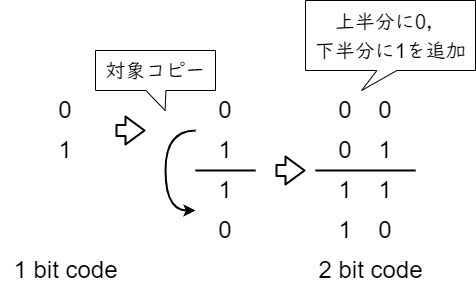
\includegraphics[width=0.4\linewidth]{gray_code.drawio.png}
    \end{center}
\end{defbox}

\begin{table}[htbp]
    \centering
    \caption{10進数の表現}
    \vspace*{-2mm}
    \begin{tabular*}{14.5cm}{wc{2.5cm} wc{2.5cm} wc{2.5cm} wc{2.5cm} wc{2.5cm}} \toprule
        10進数 & 2進数 & BCD & 3増しコード & グレイコード\\ \midrule
        0 & 0000 & 0000 & 0011 & 0000 \\
        1 & 0001 & 0001 & 0100 & 0001 \\
        2 & 0010 & 0010 & 0101 & 0011 \\
        3 & 0011 & 0011 & 0110 & 0010 \\
        4 & 0100 & 0100 & 0111 & 0110 \\
        5 & 0101 & 0101 & 1000 & 0111 \\
        6 & 0110 & 0110 & 1001 & 0101 \\
        7 & 0111 & 0111 & 1010 & 0100 \\
        8 & 1000 & 1000 & 1011 & 1100 \\
        9 & 1001 & 1001 & 1100 & 1101 \\ \bottomrule
    \end{tabular*}
    \label{tab:decimal}
\end{table}

\subsection{負数の表現}

\subsubsection{符号・絶対値表現}

MSBを0なら+,1なら-を表す符号ビットとして用いて,下位のビット列で数の絶対値を表す.
例えば,$-42_{10} = 10101011_2 \ (42_{10} = 00101011_2)$と表現できる.
4ビットの場合の10進数と2進表現の対応を\tref{tab:negative_abs}に示す.

符号なし$n$ビット2進数の場合は,$0$から$2^n-1$までの$2^n$個の数を表現できるが,
符号・絶対値表現を用いた場合はMSBを符号ビットとして用いるため,
$-(2^{n-1} - 1)$から$2^{n-1} - 1$までの$2^{n} - 1$個の数を表現できる.
\tref{tab:negative_abs}から分かるように,$0_{10}$の表現が2つ存在するため,符号なし$n$ビット2進数の場合と比較して表現できる数が1つ少ない.

\begin{table}[htbp]
    \centering
    \caption{符号・絶対値表現}
    \vspace*{-2mm}
    \begin{tabular*}{14cm}{wc{3cm} wc{3cm} wc{3cm} wc{3cm}} \toprule
        10進数 & 2進表現 & 10進数 & 2進表現 \\ \midrule
        -7 & 1111 & +0 & 0000 \\
        -6 & 1110 & +1 & 0001 \\
        -5 & 1101 & +2 & 0010 \\
        -4 & 1100 & +3 & 0011 \\
        -3 & 1011 & +4 & 0100 \\
        -2 & 1010 & +5 & 0101 \\
        -1 & 1001 & +6 & 0110 \\
        -0 & 1000 & +7 & 0111 \\ \bottomrule
    \end{tabular*}
    \label{tab:negative_abs}
\end{table}

\subsubsection{補数}

$n$進数の補数には,$n$の補数と$n-1$の補数が存在する.
それぞれ,以下のように定義されている.

\begin{exprbox}{補数}
    元の数との和が桁上りする数のうち最小のもの.\\
    例1 : $4_{10}$の補数は$6_{10}$ → $4_{10} + 6_{10} = 10_{10}$\\
    例2 : $0011_{2}$の補数は$1101_{2}$ → $0011_{2} + 1101_{2} = 10000_{2}$
\end{exprbox}

\begin{exprbox}{減基数}
    元の数との和が桁上りしない数のうち最大のもの.\\
    例1 : $4_{10}$の補数は$5_{10}$ → $4_{10} + 5_{10} = 9_{10}$\\
    例2 : $0011_{2}$の補数は$1100_{2}$ → $0011_{2} + 1100_{2} = 1111_{2}$
\end{exprbox}

2進数の場合では,2の補数と1の補数が存在する.
1の補数は元の2進数のビット反転で得られ,2の補数は1の補数に1を加えたもので得られる.



\begin{table}[htbp]
    \centering
    \caption{2の補数}
    \vspace*{-2mm}
    \begin{tabular*}{14cm}{wc{3cm} wc{3cm} wc{3cm} wc{3cm}} \toprule
        10進数 & 2進表現 & 10進数 & 2進表現 \\ \midrule
        -8 & 1000 & +0 & 0000 \\
        -7 & 1001 & +1 & 0001 \\
        -6 & 1010 & +2 & 0010 \\
        -5 & 1011 & +3 & 0011 \\
        -4 & 1100 & +4 & 0100 \\
        -3 & 1101 & +5 & 0101 \\
        -2 & 1110 & +6 & 0110 \\
        -1 & 1111 & +7 & 0111 \\ \bottomrule
    \end{tabular*}
    \label{tab:negative_2}
\end{table}

\newpage

\subsection{実数の表現}

\subsubsection{固定小数点表示}

\subsubsection{浮動小数点表示}

\section{演算制御}

\subsection{加減算器}

\subsection{乗算器}

\subsection{除算器}

\subsection{ALU}

\section{アーキテクチャ}

\section{メモリシステム}

\section{オペレーティングシステム}

\subsection{OSの役割}

\begin{enumerate}
    \item ハードウェア機構の隠蔽
    \item ハードウェア装置の管理
    \item ソフトウェア実行時の保護
\end{enumerate}

\section{プロセス管理}

ここで,プロセスとはプログラムとメモリに割り付けられるプロセス領域のことである.
イメージとしては\fref{fig:process}のような,プロセス領域の箱に格納されている任意のプログラムで,プロセス領域が異なれば,プログラムが同じでも別のプロセスとして扱われる.

\fig{0.4}{process.drawio.png}{プロセスのイメージ}{process}

プロセス管理とは,OSによって行われる次のような処理である.

\begin{itemize}
    \item プロセス状態の管理
    \item 実行しているプロセスの切り替え(プロセススイッチ) 
    \item プロセスの生成と消去
    \item プロセス実行順序の決定(プロセススケジューリング)
    \item プロセスからの実行フローの生成と管理
    \item 複数プロセスの同期
    \item 複数プロセス間の通信
\end{itemize}

\subsection{プロセス状態}

プロセスは以下の状態を持ち,\fref{fig:process_state}のように遷移する.

\begin{description}
    \item[実行中 :] プロセッサを占有している状態
    \item[実行可能 :] プロセッサを占有していないが,実行できる状態
    \item[待ち :] プロセッサを占有しておらず,実行できない状態
\end{description}

\fig{0.4}{process_state.drawio.png}{プロセス状態の遷移}{process_state}



\subsection{プロセススケジューリング}

\subsection{プロセス同期}

\subsection{プロセス間通信}



\section{メモリ管理}

\section{入出力制御}
